\documentclass[a4paper,11pt,DIV18,BCOR0mm]{scrartcl}
\usepackage[utf8]{inputenc}
\usepackage[francais]{babel}
\usepackage[T1]{fontenc}
\usepackage{amsmath}
\usepackage{amssymb}
\usepackage{color}
\usepackage{textcomp}
\usepackage[official]{eurosym}
\usepackage{enumitem}
\usepackage{numprint}
\usepackage{graphicx}
\usepackage{xifthen}
\usepackage{pifont}
%\usepackage{xlop}
\usepackage{subfig}
\usepackage{cellspace,stmaryrd}
\usepackage[french]{varioref}
\usepackage{pstricks,pst-circ,pstricks-add,pst-plot,pst-math}
%\usepackage{pst-all,pst-tree,pst-3dplot}
\RequirePackage[amsmath,thmmarks,hyperref,framed]{ntheorem}
\usepackage{mathrsfs}

% ==================================================
% Intervalles
% ==================================================
\newcommand{\intervalle}[4]{\mathopen{#1}#2\mathpunct{};#3\mathclose{#4}}
\newcommand{\intff}[2]{\intervalle{[}{#1}{#2}{]}}
\newcommand{\intof}[2]{\intervalle{]}{#1}{#2}{]}}
\newcommand{\intfo}[2]{\intervalle{[}{#1}{#2}{[}}
\newcommand{\intoo}[2]{\intervalle{]}{#1}{#2}{[}}
\newcommand{\intn}[2]{\intervalle{\llbracket}{#1}{#2}{\rrbracket}}
\newcommand{\bigintervalle}[4]{\bigl{#1}#2\mathpunct{};#3\bigr{#4}}
\newcommand{\bigintff}[2]{\bigintervalle{[}{#1}{#2}{]}}
\newcommand{\bigintof}[2]{\bigintervalle{]}{#1}{#2}{]}}
\newcommand{\bigintfo}[2]{\bigintervalle{[}{#1}{#2}{[}}
\newcommand{\bigintoo}[2]{\bigintervalle{]}{#1}{#2}{[}}
\newcommand{\bigintn}[2]{\bigintervalle{\llbracket}{#1}{#2}{\rrbracket}}
\newcommand{\Bigintervalle}[4]{\Bigl{#1}#2\mathpunct{};#3\Bigr{#4}}
\newcommand{\Bigintff}[2]{\Bigintervalle{[}{#1}{#2}{]}}
\newcommand{\Bigintof}[2]{\Bigintervalle{]}{#1}{#2}{]}}
\newcommand{\Bigintfo}[2]{\Bigintervalle{[}{#1}{#2}{[}}
\newcommand{\Bigintoo}[2]{\Bigintervalle{]}{#1}{#2}{[}}
\newcommand{\Bigintn}[2]{\Bigintervalle{\llbracket}{#1}{#2}{\rrbracket}}
\newcommand{\biggintervalle}[4]{\biggl{#1}#2\mathpunct{};#3\biggr{#4}}
\newcommand{\biggintff}[2]{\biggintervalle{[}{#1}{#2}{]}}
\newcommand{\biggintof}[2]{\biggintervalle{]}{#1}{#2}{]}}
\newcommand{\biggintfo}[2]{\biggintervalle{[}{#1}{#2}{[}}
\newcommand{\biggintoo}[2]{\biggintervalle{]}{#1}{#2}{[}}
\newcommand{\biggintn}[2]{\biggintervalle{\llbracket}{#1}{#2}{\rrbracket}}
\newcommand{\Biggintervalle}[4]{\Biggl{#1}#2\mathpunct{};#3\Biggr{#4}}
\newcommand{\Biggintff}[2]{\Biggintervalle{[}{#1}{#2}{]}}
\newcommand{\Biggintof}[2]{\Biggintervalle{]}{#1}{#2}{]}}
\newcommand{\Biggintfo}[2]{\Biggintervalle{[}{#1}{#2}{[}}
\newcommand{\Biggintoo}[2]{\Biggintervalle{]}{#1}{#2}{[}}
\newcommand{\Biggintn}[2]{\Biggintervalle{\llbracket}{#1}{#2}{\rrbracket}}

\newcommand{\pt}{.}
\newcommand{\et}{\text{ et }}
\newcommand{\si}{\text{ si }}
\newcommand{\tq}{\text{ tq }}
\newcommand{\sinon}{\text{ sinon }}
\newcommand{\avec}{\text{ avec }}
\def\pour{\text{~pour~}}

\newenvironment{enumeratecol}[1][2]{\begin{multicols}{#1}\begin{enumerate}}{\end{enumerate}\end{multicols}}


\newcommand{\set}[1]{\left\{#1\right\}}


%\newtheorem{theoreme}{Théorème}
%\newtheorem{axiome}{Axiome}
\newtheorem*{proprieteadmise}{Propriété (admise)}
%\newtheorem*{demonstration}{Démonstration}
\newtheorem*{notation}{Notation}
\newtheorem*{application}{Application}
\newtheorem*{consequence}{Conséquence}
\newtheorem{roc}{Restitution organisée de connaissances.}


\theoremstyle{plain}
\theoremheaderfont{\normalfont\bfseries}
\theorembodyfont{\normalfont}
\theoremseparator{.}
\newtheorem{exercice}{Exercice}
\newtheorem{cours}{Question de cours}
\newtheorem{probleme}{Problème}

\theoremstyle{plain}
\theoremheaderfont{\normalfont\bfseries}
\theorembodyfont{\normalfont}
\theoremseparator{.}
\newtheorem*{rappel}{Rappel}
\newtheorem{exemple}{Exemple}
\newtheorem*{contreexemple}{Contre-exemple}
\newtheorem{remarque}{Remarque}
\newtheorem*{interpretation}{Interprétation}
\newtheorem*{convention}{Convention}
\newtheorem*{vocabulaire}{vocabulaire}

\theoremheaderfont{\sc}\theorembodyfont{\upshape}
\theoremstyle{nonumberplain}
\theoremseparator{ : }
%\theoremsymbol{\rule{1ex}{1ex}}
\theoremsymbol{\ensuremath\square}
\newtheorem{demonstration}{D\'emonstration}



\usepackage[S]{thmbox}
\newtheorem[S]{theoreme}{Théorème}
\newtheorem[S]{propriete}{Propriété}
\newtheorem[S]{axiome}{Axiome}
\newtheorem[S]{methode}{Méthode de résolution}
\newtheorem[L]{definition}{Définition}

\newcommand{\defi}[1]{
\begin{definition}
#1
\end{definition}
}

\newcommand{\theo}[1]{
\begin{theoreme}
#1
\end{theoreme}
}

\newcommand{\demo}[1]{
\begin{demonstration}
#1
\end{demonstration}
}


%-------------------------------------------------
%         TYPOGRAPHIE
%-------------------------------------------------
\newcommand{\celsius}{\,\degres\textrm{C}}


%-------------------------------------------------
%         SCOLAIRE
%-------------------------------------------------
\newcommand{\trou}[1]{\textcolor{white}{#1}}
\newcommand{\prof}[1]{\textcolor{blue}{#1}}
\newcommand{\exercices}[1]{\begin{flushright}\textbf{Exercices : }#1\end{flushright}}

\newcommand{\np}[1]{\numprint{#1}}

\newcommand{\place}[1]{
\vfill\begin{center}
< #1>
\end{center}
\vfill
}

\newif\ifeleve
\def\ac#1{\ifeleve%
\setbox1\hbox{#1}%
\lower2pt\hbox to \wd1{\dotfill}%
\else#1\fi}

\newcommand{\croi}{% croissante
\unitlength=1cm
\begin{minipage} {1cm}%pour centrer verticalement f(x)
\begin{picture}(1,1) % dessin de 2 X 2
\put(0,0){\vector(1,1){1}} % 1 à partir (0,0) direction (1,1)
\end{picture}
\end{minipage}
}
\newcommand{\dec}{%décroissante
\unitlength=1cm
\begin{minipage} {1cm}%pour centrer verticalement f(x)
\begin{picture}(1,1) % dessin de 2 X 2
\put(0,1){\vector(1,-1){1}}
\end{picture}
\end{minipage}
} 

\newcommand{\tauxfxh}[3]{\dfrac{#1(#2+#3)-#1(#2)}{#3}}

\newcounter{QCM}
\setcounter{QCM}{1}
\newcommand{\question}[1]{{\item[Question \arabic{QCM}]\addtocounter{QCM}{1}#1}}
\newcommand{\choix}[3]{
\[
 \begin{tabular}{p{5cm}p{5cm}p{5cm}}
  \textbf{a) }#1.&\textbf{b) }#2.&\textbf{c) }#3.
 \end{tabular}
\]
}

%-------------------------------------------------
%         GEOMETRIE
%-------------------------------------------------
\newcommand{\vect}{\overrightarrow}
\newcommand{\norme}[1]{\|#1\|}
\newcommand{\Norme}[1]{\left\|#1\right\|}
\newcommand{\Oijk}{(O,\vect{i},\vect{j},\vect{k})}
\newcommand{\Oij}{(O,\vect{i},\vect{j})}
\newcommand{\Ouv}{(O,\vect{u},\vect{v})}
\newcommand{\bary}{\mathrm{Bar}}

%-------------------------------------------------
%         FONCTIONS
%-------------------------------------------------
\newcommand{\donne}{\mapsto}
\newcommand{\dx}{\mathrm{d}x}
\newcommand{\dt}{\mathrm{d}t}
\newcommand{\intab}{\int_{a}^{b}}
%-------------------------------------------------
%         PROBA
%-------------------------------------------------
\newcommand{\barre}[1]{\overline{#1}}

%-------------------------------------------------
%         ALGEBRE LINEAIRE
%-------------------------------------------------
\newcommand{\rg}{\text{rg}}
\newcommand{\tr}{\text{tr}}
\renewcommand{\Im}{\text{Im}}
\newcommand{\Vect}{\text{Vect}}
\newcommand{\LL}{\mathcal{L}}
\newcommand{\FF}{\mathcal{F}}
\newcommand{\MM}{\mathcal{M}}
\newcommand{\transpose}{{}^{t}}
%\newcommand{\ker}{\text{ker}}
\newcommand{\coordo}[2]{
\begin{pmatrix}
#1 \\ #2
\end{pmatrix}
}

%-------------------------------------------------
%         ARITHMETIQUE
%-------------------------------------------------
\newcommand{\congru}{\equiv}

%-------------------------------------------------
%         NOMBRES COMPLEXES
%-------------------------------------------------
\newcommand{\e}{\mathrm{e}}
\newcommand{\ii}{\mathrm{i}}
\newcommand{\ei}[1]{\mathrm{e}^{\ii#1}}
\newcommand{\C}{\mathbb{C}}
\newcommand{\U}{\mathbb{U}}
\newcommand{\re}[1]{\mathrm{Re}(#1)}
\newcommand{\im}[1]{\mathrm{Im}(#1)}
\newcommand{\conj}[1]{\overline{#1}}
\newcommand{\abs}[1]{\left\lvert#1\right\rvert}
\renewcommand{\arg}[1]{\mathrm{Arg}(#1)}

\newcommand{\pparmin}[2]{\binom{#2}{#1}}
\newcommand{\Pparmin}[2]{\dbinom{#2}{#1}}

\newcommand{\R}{\mathbb{R}}
\newcommand{\K}{\mathbb{K}}
\newcommand{\N}{\mathbb{N}}
\newcommand{\Z}{\mathbb{Z}}
\newcommand{\D}{\mathbb{D}}
\newcommand{\Q}{\mathbb{Q}}
\newcommand{\rond}{\circ}
\newcommand{\repereoij}{repère orthonormal $(O,\vect{i},\vect{j})$}
\newcommand{\repereoijdirect}{repère orthonormal direct $(O,\vect{i},\vect{j})$}
\newcommand{\accoladedouble}[2]{\left\{\begin{array}{ll}#1\\#2\end{array}\right.}
\newcommand{\soitlasuite}[4]{Soit $(#1)$ la suite définie par $\accoladedouble{#2}{#3\text{ pour tout $#4$}}$}
\newcommand{\coordvect}[2]{\left(\begin{array}{c}#1\\#2\end{array}\right)}
\newcommand{\baremeexo}[1]{\marginpar{\textbf{(#1)}}}
\newcommand{\baremeque}[1]{\marginpar{(#1)}}
\newcommand{\bq}[1]{\marginpar{\textcolor{red}{(#1)}}}


\newcommand{\less}{\leqslant}
\newcommand{\more}{\geqslant}
\newcommand{\equi}{\Longleftrightarrow}
\newcommand{\implique}{\Rightarrow}
\newcommand{\equidef}{\stackrel{def}{\Longleftrightarrow}}
\newcommand{\ssi}{\Longleftrightarrow}
\newcommand{\eqdef}{\stackrel{def}{=}}
\newcommand{\egaldef}{\stackrel{\tiny{def}}{=}}
\newcommand{\egalnot}{\stackrel{\tiny{notation}}{=}}
\newcommand{\latin}[1]{\emph{#1}}
\newcommand{\negl}[1]{\underset{\text{\tiny{$#1$}}}{\ll}}

\newcommand{\limsuite}{\displaystyle\lim_{n\to+\infty}}

% Partie à ommettre en première lecture
\newcommand{\optionnel}[1]{\noindent\hrulefill \rotatebox{180}{\ding{72}\ding{72}\ding{72}} \hrulefill #1 \noindent\hrulefill \ding{72}\ding{72}\ding{72} \hrulefill}
% En tête et pieds custom
\usepackage{fancyhdr}
\pagestyle{fancy}
\lhead{\today}
\rhead{Cours}		
\lfoot{\tiny{vg}}
\cfoot{}
\rfoot{\tiny{Lycée Émile Loubet, Valence}}


% de Dupuy de lome
%\newcommand{\norme}[1]{\left\lVert\ifempty{#1}{\dotpourvariable}{#1}\right\rVert}
\newcommand{\bignorme}[1]{\bigl\lVert#1\bigr\rVert}
\chead{}
\lhead{2\up{nde}3, 2017-2018}
\rhead{Généralités sur les fonctions}
\rfoot{\tiny{Lycée Émile Loubet, Valence}}
\lfoot{}
\cfoot{}

\begin{document}
\section{Notion de fonction}
Une fonction est une correspondance \og un $\longrightarrow$ au plus un\fg{}
entre deux ensembles : à chaque élément de l'ensemble de départ, elle fait correspondre 
au plus un élément de l'ensemble d'arrivée.

Exemple : relevé des notes sur 10 obtenues par 8 élèves d'une même classe (A, B, C, D, E, F, G, H) :
\[
\begin{array}{c|c|c|c|c|c|c|c}
 A&B&C&D&E&F&G&H\\\hline
 3&7&5&Absent&6&8&8&4
\end{array}
\]
\vfill\begin{center}
< Diagramme avec le vocabulaire : Ensemble de départ, ensemble de définition, ensemble d'arrivée,
\textbf{un} antécédent de , \textbf{l}'image de.>
\end{center}
\vfill
Remarque : ce qui est important, c'est qu'un élément de l'ensemble de départ ne puisse jamais correspondre 
à deux éléments différents de l'ensemble d'arrivée. Dans ce cas, la correspondance n'est pas une fonction.

Exemple : $f:x\donne 3x+2$.

\exercices{7 à 12 p. 26}

\pagebreak
\section{Nombres réels, fonctions numériques}
Les fonctions du lycée sont des fonctions numériques, cela veut dire que l'ensemble de départ est un ensemble de nombres
et que l'ensemble d'arrivée est un ensemble de nombres.

\subsection{La droite réelle}
L'\og ensemble de tous les nombres\fg connus en seconde est noté $\R$ et appelé l'ensemble des nombres réels. Il peut être représenté par une droite :

\place{droite réelle}.


\begin{exemple}
Nombres réels : les nombres entiers, les nombres qui ont
un développement décimal fini, les fractions (ou nombres rationnels)
qui ont un dévelopement décimal périodique,
et encore d'autres : $\sqrt{2}$, $\frac{1+\sqrt{3}}{2}$,
$\pi$, etc.
\end{exemple}


\subsection{Intervalle de $\R$}
Les intervalles de $\R$ sont les parties de
$\R$ qui correspondent
aux segments et aux demi-droites de la droite réelles,
éventuellement privés de leurs extrémités.
\begin{exemple}

\end{exemple}

\begin{definition}
Soit $a$ et $b$ deux nombres réels avec $a\leq b$.
L'intervalle $[a;b]$ est l'ensemble des nombres réels $x$
tels que $a\leq x\leq b$.
\end{definition}


\exercices{13, 14, 15, 16 p. 27}


\pagebreak
\section{Différentes manières de donner la correspondance entre $x$ et $f(x)$}
On peut définir une fonction par un tableau ou un diagramme, comme dans la première partie.
On définit également parfois des fonctions par leur représentation graphique, mais la manière la plus importante 
de définir une fonction
en mathématiques au lycée est de la définir par une formule.

\subsection{Fonction définie par une formule (ou un algorithme)}
Il s'agit de décrire une succession de calculs à effectuer avec l'antécédent 
pour obtenir l'image.
\begin{exemple}
 Soit $f$ la fonction définie sur $\R$ par :
\[
 f(x)=2x+3.
\]
\begin{enumerate}
 \item Déterminer l'image de 5 par $f$.
 \item Calculer $f(10)$.
 \item Quels sont les antécédents de 11 par $f$ ?
 \item Résoudre $f(x)=15$.
\end{enumerate}
\end{exemple}
Notation : on peut aussi définir la même fonction $f$ en écrivant simplement : 
\[
 \begin{array}{cccc}
  f:&\R&\rightarrow&\R\\
    &x&\donne&2x+3
 \end{array}
\]
\exercices{33, 34, 35, \textbf{36} p 44, TP 1 p  37}

\subsection{Fonction \og définie\fg{} par un problème}
Beaucoup de situations concrètes peuvent être modélisées par des fonctions.
Dans ce cas, la question sera souvent de la forme : \og Exprimer <nom de la grandeur à l'arrivée>
en fonction de <nom de la grandeur au départ>\fg.

Exemples :

\begin{itemize}
 \item Exprimer l'angle au sommet $s$ d'un triangle isocèle en fonction de son angle à la base $x$.
 \item Un magasin fait une réduction de 10\% sur tous ses articles. Exprimer le nouveau prix $n$ en fonction de l'ancien prix $x$.
 \item D'après la loi d'Ohm, $U=RI$. Exprimer l'intensité en fonction de la tension aux bornes d'un resistance de $10~\Omega$.
\end{itemize}


\subsection{Représentation graphique}
\begin{exemple}
Le graphique ci-dessous définit (à la précision de la lecture graphique près) la fonction $f$ (température) en fonction
de l'heure de la journée $x$.
 \[
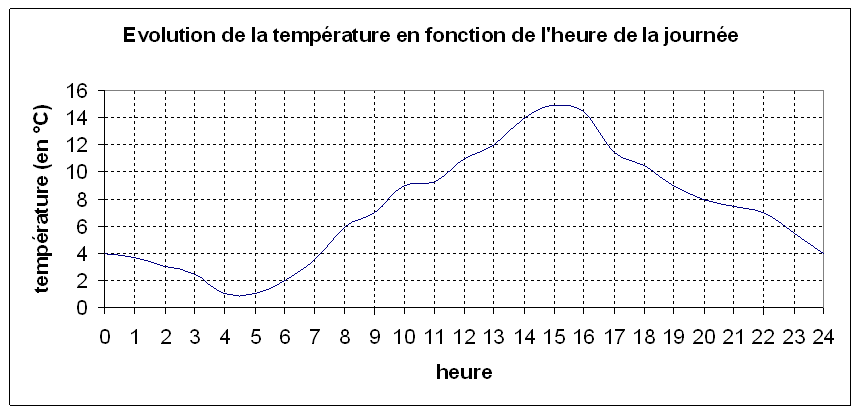
\includegraphics[width=0.8\textwidth]{fonction_temperature}
\]
L'ensemble de définition est l'intervalle $[0,24]$.
\begin{enumerate}
 \item Déterminer par lecture graphique l'image de 20 par $f$.
 \item Déterminer $f(13)$ par lecture graphique.
 \item Par lecture graphique, déterminer l'ensemble des antécédents de 2 par $f$.
 \item Le nombre 16 a-t-il des antécédents par $f$ ?
\end{enumerate}
\exercices{46, 47     p  46,  TP 5 p 41}
\end{exemple}

\begin{definition}
 Soit $f$ une fonction définie sur un intervalle $I$ de $\R$. La représentation graphique
de $f$ dans un repère est l'ensemble des points $M(x,y)$ dont les coordonnées vérifient
\[
 y=f(x).
\]
\end{definition}

\section{Variations d'une fonction}
\subsection{Définitions}
\subsection{Tableaux de variation}




\end{document}

